%% -*- TeX-engine: luatex; ispell-language: "russian" -*-

\documentclass[a4paper,12pt]{article}

\usepackage[left=1.5cm,right=2cm,top=1.5cm,bottom=2cm]{geometry}

\usepackage{parskip}
\setlength{\parindent}{0mm}
\setcounter{secnumdepth}{1}

\usepackage{amsmath}

\usepackage{graphicx}

\usepackage{fontspec}
\setmainfont{PT Serif}
\newfontfamily\cyrillicfont[Script=Cyrillic,Ligatures=TeX]{PT Serif}
\setsansfont{PT Sans}
\setmonofont[Ligatures=NoCommon]{PT Mono}
\defaultfontfeatures{Ligatures=TeX}

\usepackage[bold-style=ISO]{unicode-math}
\setmathfont{XITS Math}

\usepackage{microtype}

\usepackage{hyperref}

\usepackage{polyglossia}
\setmainlanguage{russian}
\setotherlanguage{english}

\usepackage{csquotes}

%% for code snippets
\usepackage{minted}
\newminted[pycon]{pycon}{fontsize=\footnotesize}
\newminted[python3]{python3}{fontsize=\footnotesize}
\newminted[bash]{bash}{fontsize=\footnotesize}
\newmintinline[pythoninline]{python3}{fontsize=\footnotesize}
\newmintinline[bashinline]{bash}{fontsize=\footnotesize}

\pagestyle{empty}


\begin{document}
\subsection*{Домашнее задание №1: <<Соседи и вино>>}

\begin{tabular}{@{}lr}
  \textbf{Дедлайн 1} (20 баллов): & 26 февраля, 23:59 \\
  \textbf{Дедлайн 2} (10 баллов): & 5 марта, 23:59
\end{tabular}

Домашнее задание нужно написать на языке Python и сдать в виде одного файла.
Правило именования файла: \texttt{name\_surname\_1.py}. Например, если
вас зовут Иван Петров, то имя файла должно быть: \texttt{ivan\_petrov\_1.py}.

\makebox[\linewidth]{\hrulefill}

В этом задании предлагается опровергнуть миф про то, что все вина на вкус
одинаковые, и заодно разобраться с классификатором k-ближайших соседей. По ссылке%
\footnote{\url{https://gist.github.com/ktisha/25e6d5a79628d19cd4b0908cd0fd2459}}
находятся данные, описывающие химический состав трёх вин из некоторого региона
Италии. Первая колонка каждой строки --- идентификатор вина, который может быть
равен 1, 2 или 3. Значения остальных колонок указаны в заголовке файла.

\paragraph{1} Прежде чем приступить к написанию классификатора, реализуйте
функцию разбиения выборки на обучающую и тестовую. Функция должна принимать
прочитанные из файла данные: матрицу признаков $X$, вектор меток класса $y$ и
соотношение, в котором нужно разбить выборку.

На Python функцию можно записать так:
\begin{python3}
def train_test_split(X, y, ratio):
    # ...
    return X_train, y_train, X_test, y_test
\end{python3}

Результат функции должен удовлетворять условию
\begin{python3}
len(X_train) / (len(X_test) + len(X_train)) == ratio
len(y_train) / (len(y_test) + len(y_train)) == ratio
\end{python3}


\paragraph{2} Классификатор k-ближайших соседей не предполагает отдельной
процедуры обучения, поэтому сразу перейдём к функции, предсказывающей метки
класса по известным примерам. Функция \pythoninline{knn} должна принимать:
\begin{itemize}
\item обучающую выборку \pythoninline{X_train}, \pythoninline{y_train},
\item выборку, которую нужно классифицировать, \pythoninline{X_test},
\item количество соседей \pythoninline{k} и
\item функцию расстояния \pythoninline{dist}, например, Евклидово расстояние.
\end{itemize}

Выходом функции является вектор \pythoninline{y_test}, в котором для каждого
элемента \pythoninline{X_test} хранится соответствующий ему класс.

\clearpage

\paragraph{3} Самое время оценить качество получившегося классификатора в
терминах точности (\emph{precision}) и полноты (\emph{recall}). Формально эти
метрики определяются следующим образом:
$$
\operatorname{Precision} = \frac{TP}{TP + FP}
\qquad
\operatorname{Recall} = \frac{TP}{TP + FN}
$$

Здесь
\begin{itemize}
\item $TP$ --- это количество элементов, которые классификатор верно отнёс к классу $c$,
\item $FP$ --- количество элементов, которые классификатор неверно отнёс к классу $c$,
\item $FN$ --- количество элементов, которые классификатор неверно отнёс к классу, отличному от $c$.
\end{itemize}

Реализуйте функцию, вычисляющую для каждого класса точность и полноту по
полученным от \pythoninline{knn} предсказаниям. На Python функцию можно записать
так:
\begin{python3}
# Обозначим за y_pred результат работы k-ближайших соседей на тестовой
# выборке X_test.
y_pred = knn(X_train, y_train, X_test, k=..., dist=...)

def print_precision_recall(y_pred, y_test):
    # Подсказка: значение n_classes можно вычислить по y_test
    #     n_classes = len(set(y_test))
    # или
    #     import numpy as np
    #     n_classes = len(np.unique(y_test))
    for c in range(n_classes):
        # ...
        print(class, precision, recall)
\end{python3}


\paragraph{4} Реализуйте функцию для выбора оптимального значения k по методу
LOO (leave one out) кросс-валидации. Функция должна принимать обучающую выборку
и функцию расстояния:
\begin{python3}
  def loocv(X_train, y_train, dist):
      # ...
      return opt_k
\end{python3}


\paragraph{5} Оцените точность и полноту предсказаний классификатора с
оптимальным k и двумя любыми функциями расстояния. Правда ли, что все вина
одинаковые?

\bigbreak
\begin{center}
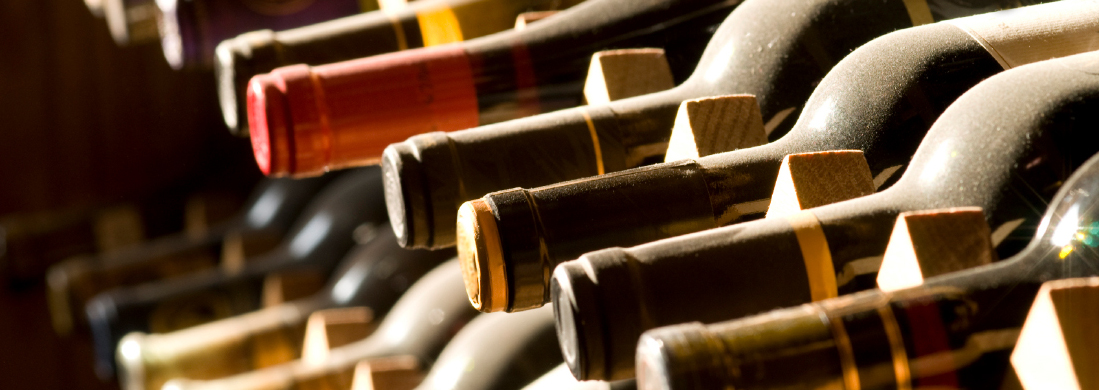
\includegraphics[width=\textwidth, keepaspectratio]{images/wine}
\end{center}


\end{document}
